\documentclass[xcolor=dvipsnames,10pt]{beamer}

\usetheme[presnum=02]{u18fest}
\usepackage{ifthen}
\usepackage{pgfplotstable}
\usetikzlibrary{positioning,fit,backgrounds,calc,math}

\subtitle{Marco Bayesiano para el análisis de datos,\\
  calibración de parámetros y modelamiento inverso}
\title{Introducción a la\\
  Teoría de Probabilidades}%
\institute{Universidad Industrial de Santander}%
\date{U18 Fest}

\tikzset{onslide/.code args={<#1>#2}{%
  \only<#1>{\pgfkeysalso{#2}} % \pgfkeysalso doesn't change the path
}}

\begin{document}

\begin{frame}[noframenumbering]
  \titlepage
\end{frame}

\begin{frame}
  \frametitle{Ud. es el modelador}
  \begin{itemize}
  \item Como toda teoría matemática, la teoría de probabilidades no representa realidades físicas. 
    En cambio, es útil para representar conceptos
  \item Nuestro objetivo es \emph{modelar} información de manera consistente y fácil de interpretar
  \item El modelador, ud., juega un rol fundamental
  \end{itemize}
\end{frame}
%
\begin{frame}
  \frametitle{Elementos de la teoría probabilidades}
  \vskip-8mm
  \begin{figure}
    \centering
    \begin{tikzpicture}[every node/.style={fill=u18fred, shape=rectangle, minimum width=0.4\textwidth, minimum height=0.3\textheight, align=center, inner sep=4mm, node distance=4mm]}]
      \node (resultados) {\textbf{Resultados}\\$\Omega$};
      \node [right=of resultados] (variables) {\textbf{Variables aleatorias}\\$X \colon \Omega \to C$};
      \node [below=of resultados] (eventos) {\textbf{Eventos}\\$\mathcal{F}$};
      \node [right=of eventos] (probabilidades) {\textbf{Probabilidades}\\$P \colon \mathcal{F} \to [0, 1]$};
      \begin{scope}[on background layer]
        \node [fill=u18fblue, fit={(resultados) (eventos) (variables) (probabilidades)}, label={[label distance=-8mm]above:\textbf{Experimento}}] (experimento) {};
      \end{scope}
    \end{tikzpicture}
  \end{figure}
\end{frame}
%
\begin{frame}
  \frametitle{Resultados}
  \begin{tcolorbox}
    \textbf{Resultado}: \emph{Posible resultado de un experimento aleatorio}
    \tcblower
    $\Omega$: \emph{Espacio} de resultados
  \end{tcolorbox}
  \emph{Ejemplos}
  \begin{itemize}
  \item Lanzar una moneda\\
    \begin{equation*}
      \Omega = \{\text{cara}, \text{sello} \}
    \end{equation*}
  \item Lanzar un dado\\
    \begin{equation*}
      \Omega = \{1, 2, 3, 4, 5, 6 \}
    \end{equation*}
  \item Lanzar dos monedas\\
    \begin{equation*}
      \Omega = \{(\text{cara}, \text{cara}), (\text{cara}, \text{sello}), (\text{sello}, \text{cara}), (\text{sello}, \text{sello}) \}
    \end{equation*}
  \end{itemize}
\end{frame}
%
\begin{frame}
  \frametitle{Resultados}
  El espacio de resultados puede ser...
  \begin{itemize}
  \item \textbf{Finito contable}\\
    \emph{Ejemplo}: Elegir un número de $1$ a $10$
    \begin{equation*}
      \Omega = \{1, 2, 3, \dots, 10 \}
    \end{equation*}
  \item \textbf{Infinito contable}\\
    \emph{Ejemplo}: Elegir un número de $0$ a infinito
    \begin{equation*}
      \Omega = \mathbb{N}^0 = \{ 0, 1, 2, \dots\}
    \end{equation*}
  \item \textbf{Incontable}\\
    \emph{Ejemplo}: Elegir un número real no negativo
    \begin{equation*}
      \Omega = \mathbb{R}^+ = [0, \infty)
    \end{equation*}
  \end{itemize}
\end{frame}
%
\begin{frame}
  \frametitle{Variables aleatorias}
  \begin{definicion*}{Funciones}{}
    La notación
    \begin{equation*}
      f \colon A \to B
    \end{equation*}
    define la función $f(\cdot)$ que asigna un elemento de $B$ a un elemento $A$.  E.g., $f(a) = b$ indica que la función asocia $b \in B$ a $a \in A$
  \end{definicion*}
\end{frame}
%
\begin{frame}
  \frametitle{Variables aleatorias}
  \begin{tcolorbox}
    \emph{Funciones de los resultados que representan cantidades asociadas al resultado del experimento}
    \tcblower
    \begin{equation*}
      X \colon \Omega \to C
    \end{equation*}
  \end{tcolorbox}
  \emph{Ejemplos}
  \begin{itemize}
  \item Lanzar dos dados
    \begin{gather*}
      \Omega = \{ (1, 1), (1, 2), (1, 3), \dots, (2, 1), (2, 2), \dots (6, 6) \}\\
      \omega \in \Omega, \quad \omega = (\omega_1, \omega_2)
    \end{gather*}
    Variable aleatoria: Suma de los dos dados
    \begin{equation*}
      X \colon \Omega \to \mathbb{N}, \quad X(\omega) = \omega_1 + \omega_2
    \end{equation*}
  \end{itemize}
\end{frame}
%
\begin{frame}
  \frametitle{Variables aleatorias}
  \emph{Ejemplos}
  \begin{itemize}
  \item Suma de dos dados: $X \colon \Omega \to \mathbb{N}$, $X(\omega) = \omega_1 + \omega_2$
    \vskip1em
    \begin{figure}
      \centering
      \def\szx{0.75cm}%
      \def\szy{0.75cm}
      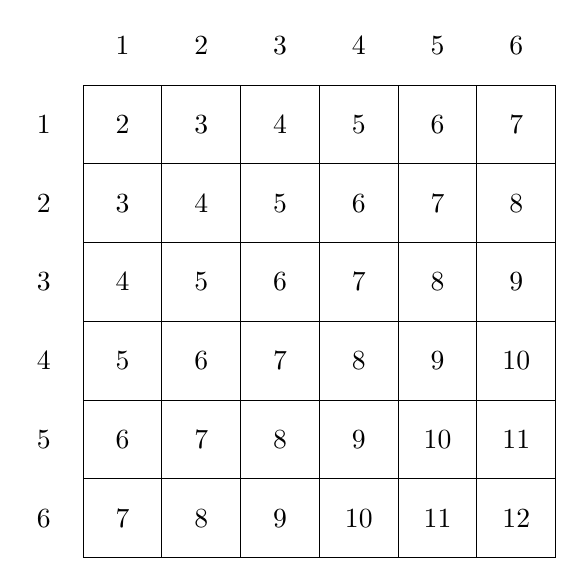
\begin{tikzpicture}
        \foreach \x in {1,...,6}{%
          \node at ($ -\x*(0,\szy) + 0.5*(0, \szy) + 0.5*(\szx, 0)$) {\x};
        }%
        \foreach \y in {1,...,6}{%
          \node at ($ \y*(\szx,0) + 0.5*(0, \szy) + 0.5*(\szx, 0)$) {\y};
        }%
        \foreach \x in {1,...,6}{%
          \foreach \y in {1,...,6}{%
            \pgfmathsetmacro\z{int(\x+\y)}%
            \draw [draw=black] ($ -\x*(0,\szy) + \y*(\szx,0) $) rectangle+(\szx,\szy);%
            \node at ($ -\x*(0,\szy) + \y*(\szx,0) + 0.5*(\szx, \szy)$) {\z};%
          }%
        }
      \end{tikzpicture}
    \end{figure}
  \end{itemize}
\end{frame}
%
\begin{frame}
  \frametitle{Variables aleatorias}
  Pueden ser \emph{discretas} o \emph{contínuas}
  \emph{Ejemplo:} Altura, ingreso y género de una población
  \begin{equation*}
    \Omega = \{ \text{personas en la población} \}
  \end{equation*}
  \begin{itemize}
  \item \textbf{Discreta}: Género
    \begin{equation*}
      G \colon \Omega \to \{ \text{masc.}, \text{fem.}, \dots \}
    \end{equation*}
  \item \textbf{Contínua}: Altura
    \begin{equation*}
      A \colon \Omega \to \mathbb{R}
    \end{equation*}
  \item Ingreso: Variable contínua o discreta?
  \end{itemize}
\end{frame}
%
\begin{frame}
  \frametitle{Eventos}
  \begin{tcolorbox}
    \textbf{Evento}: \emph{Subconjunto de resultados del experimento}
    \tcblower
    $\mathcal{F}$: \emph{Campo} de eventos
  \end{tcolorbox}
  \begin{definicion*}{Conjunto-poder}{}
    Para $\Omega$ \emph{contable}, una selección común de campo de eventos es el conjunto-poder $2^{\Omega}$, que contiene los siguientes eventos:
    \begin{itemize}
    \item Cada resultado (evento elemental)
    \item Todos los subconjuntos de $\Omega$
    \item Todos los resultados (osea $\Omega$)
    \item Ningún resultado (conjunto vacío, $\varnothing$)
    \end{itemize}
  \end{definicion*}
\end{frame}
%
\begin{frame}
  \frametitle{Eventos}
  \emph{Ejemplo}: Lanzar un dado
  \begin{equation*}
    \Omega = \{1, 2, 3, 4, 5, 6 \}
  \end{equation*}
  Algunos eventos en el conjunto-poder $\mathcal{F} = 2^{\Omega}$:
  \begin{columns}
    \begin{column}{0.48\textwidth}
      \begin{itemize}
      \item El número 3
      \item Un número par
      \item Un número menor a 4
      \end{itemize}
    \end{column}
    \begin{column}{0.48\textwidth}
      \begin{itemize}
      \item Un número entre 2 y 5
      \item Cualquier número ($\Omega$)
      \item Ningún número ($\varnothing$)
      \end{itemize}
    \end{column}
  \end{columns}
\end{frame}
%
\begin{frame}
  \frametitle{Eventos}
  \uncover<3->{También es posible definir eventos en términos de los valores de variables aleatorias}
  \vskip1em
  \emph{Ejemplo}: Lanzar dos dados\uncover<3>{, suma $X(\omega) = \omega_1 + \omega_2$}
  \begin{columns}
    \begin{column}{0.48\textwidth}
      \begin{figure}
        \centering%
        \def\szx{0.75cm}%
        \def\szy{0.75cm}
        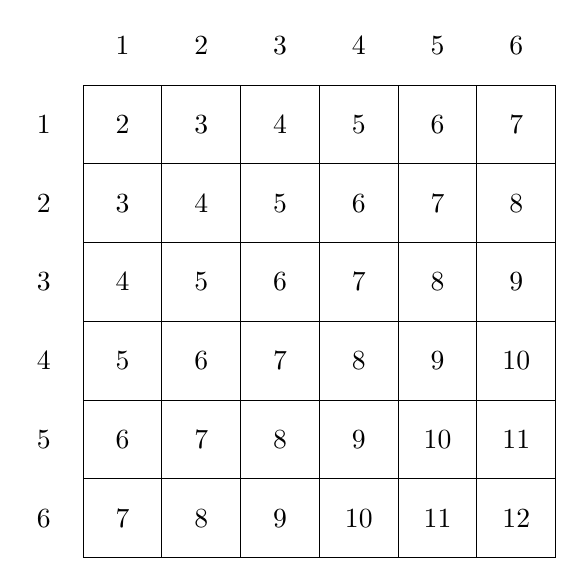
\begin{tikzpicture}
          \foreach \x in {1,...,6}{%
            \node at ($ -\x*(0,\szy) + 0.5*(0, \szy) + 0.5*(\szx, 0)$) {\x}; }%
          \foreach \y in {1,...,6}{%
            \node at ($ \y*(\szx,0) + 0.5*(0, \szy) + 0.5*(\szx, 0)$) {\y}; }%
          \foreach \x in {1,...,6}{%
            \foreach \y in {1,...,6}{%
              \pgfmathsetmacro\z{int(\x+\y)}%
              \pgfmathsetmacro\ncola{and(\x <= 4, \y <= 4) ? "u18fred": "white"}%
              \pgfmathsetmacro\ncolb{or(\x < 3, \x > 5) ? "u18fred": "white"}%
              \pgfmathsetmacro\ncolc{\z >= 7 ? "u18fred": "white"}%
              \pgfmathsetmacro\ncold{and(\z >=7, \y >= 3) ? "u18fred": "white"}%
              \draw [onslide=<1>{fill=\ncola}, onslide=<2>{fill=\ncolb}, onslide=<3>{fill=\ncolc}, , onslide=<4>{fill=\ncold}] ($ -\x*(0,\szy) + \y*(\szx,0) $) rectangle+(\szx,\szy);%
              \node at ($ -\x*(0,\szy) + \y*(\szx,0) + 0.5*(\szx, \szy)$) {\z};%
            }%
          }
        \end{tikzpicture}
      \end{figure}
    \end{column}
    \begin{column}{0.48\textwidth}
      \only<1>{Ambos dados menor o igual a $4$}%
      \only<2>{%
        Dado \# 1...
        \begin{itemize}
        \item $E_1$: Menor a 3
        \item $E_2$: Mayor a 6
        \end{itemize}
        \vskip1em
        Eventos $E_1$ y $E_2$ son \emph{Mutuamente excluyentes}
        }
      \only<3>{Suma $X$ mayor o igual a 7}
      \only<4>{%
        Suma mayor o igual a $7$, pero el dado \# 2 es $3$ o mayor%
      }
    \end{column}
  \end{columns}
\end{frame}
%
\begin{frame}
  \frametitle{Probabilidades}
  \begin{definicion*}{Axiomas de probabilidades}{}
    Las probabilidades son...
    \begin{enumerate}
    \item ... cantidades reales no negativas asociadas a cada evento en $\mathcal{F}$...
      \begin{equation*}
        P \colon \mathcal{F} \to \mathbb{R}^+
      \end{equation*}
    \item ... aditivas sobre eventos mutuamente exclusivos
      \begin{equation*}
        \text{Si } A \cap B = \varnothing \text{, entonces } P(A \cup B) = P(A) + P(B)
      \end{equation*}
    \item ... que suman a $1$ sobre el conjunto de resultados
      \begin{equation*}
        P(\Omega) = 1
      \end{equation*}
    \end{enumerate}
  \end{definicion*}
  \pause
  Los axiomas implican que $0 \leq P(E) \leq 1$ para $E \in \mathcal{F}$
\end{frame}
%
\begin{frame}
  \frametitle{Probabilidades}
  \emph{Ejemplo}: Lanzar dos dados, suma $X(\omega) = \omega_1 + \omega_2$
  \begin{columns}
    \begin{column}{0.48\textwidth}
      \begin{figure}
        \centering%
        \def\szx{0.75cm}%
        \def\szy{0.75cm}
        \begin{tikzpicture}
          \foreach \x in {1,...,6}{%
            \node at ($ -\x*(0,\szy) + 0.5*(0, \szy) + 0.5*(\szx, 0)$) {\x}; }%
          \foreach \y in {1,...,6}{%
            \node at ($ \y*(\szx,0) + 0.5*(0, \szy) + 0.5*(\szx, 0)$) {\y}; }%
          \foreach \x in {1,...,6}{%
            \foreach \y in {1,...,6}{%
              \pgfmathsetmacro\z{int(\x+\y)}%
              \pgfmathsetmacro\ncol{\z >= 7 ? "u18fred": "white"}%
              \draw [fill=\ncol] ($ -\x*(0,\szy) + \y*(\szx,0) $) rectangle+(\szx,\szy);%
              \node at ($ -\x*(0,\szy) + \y*(\szx,0) + 0.5*(\szx, \szy)$) {\z};%
            }%
          }
        \end{tikzpicture}
      \end{figure}
    \end{column}
    \begin{column}{0.48\textwidth}
      \begin{itemize}
      \item $E_i$, $i \in [1, 36]$: Eventos elementales
      \item $P(E_i) = 1 / 36 \approx 2.8\%$
        \item $P(X \geq 7) = 21 / 36 \approx 58\%$
      \end{itemize}
    \end{column}
  \end{columns}
\end{frame}
%
\begin{frame}
  \frametitle{Probabilidades}
  \begin{itemize}
  \item Hasta ahora probabilidades se han definido de manera enteramente \emph{abstracta}
  \item Probabilidad es una \emph{medida}: ``Área'' asociada a una región del espacio de resultados (Evento)
  \item Qué significa que un evento tenga probabilidad de $58 \%$?
  \end{itemize}
\end{frame}
%
\begin{frame}
  \frametitle{Probabilidades}
  \begin{itemize}
  \item Interpretación \emph{frecuentista}: Si el experimento se ejecuta $n$ veces, se observará un $58 \%$ de las veces el evento en cuestión
    \pause
  \item Cuál es la interpretación adecuada para la probabilidad de eventos que sólo ocurren una vez?
  \item E.g. el evento ``llover mañana'': Sólo hay --un-- mañana!
    \pause
  \item \textbf{Probabilidades como medida de (in)certidumbre}
  \end{itemize}
\end{frame}
%
\begin{frame}
  \frametitle{Eventos asociados a variables aleatorias contínuas}
  Considérese la variable aleatoria
  \begin{equation*}
    A \colon \Omega \to \mathbb{R}
  \end{equation*}
  Qué eventos podemos definir en términos de los valores de $A$?
  \vskip1em\pause
  Para cierto valor $a$...
  \begin{itemize}
  \item $P(A = a)$? \pause\\\alert<3>{En general, $A = a$ es un evento con probabilidad trivial $(= 0)$}\pause
  \item $P(A \leq a)$, $P(A > a)$, $P(a \leq A \leq b)$, etc.
    \pause
  \item Revisaremos éste aspecto luego
  \end{itemize}
\end{frame}

\end{document}

%%% Local Variables:
%%% TeX-master: t
%%% TeX-engine: luatex
%%% ispell-local-dictionary: "es_CO"
%%% End:
